\section{Vector Field Topology}


\subsection{Vector Fields as ODEs}
What are conditions for existence and uniqueness of streamlines?

\begin{description}
    \item For the initial value problem
        \begin{align*}
            \dot x(t) &= v(x(t)) &x(t_0) = x_0
        \end{align*}
        a solution \emph{exists} if the velocity field $v(x)$ is \emph{continuous}.
    \item The solution is \emph{unique} if the field is \emph{Lipschitz}-continuous, i.e. if there is a constant $M$ such that 
        \begin{align*}
            \norm{v(x)-v(x')} &\leq M\norm{x-x'} & \forall x,x' \in \R.
        \end{align*}
\end{description}

Lipschitz-continuous is strong than continuous ($C^0$) but weaker than continuously differentiable ($C^1$).

Important for scientific visualisation:
\begin{itemize}
    \item \emph{Piecewise multilinear} functions are Lipschitz-continuous,
    \item \emph{cellwise} bi- or trilinear interpolation is Lipschitz-continuous.
\end{itemize}

Consequence: \emph{Numerical} vector fields do have unique streamlines, but \emph{analytic} vector fields don't necessarily.

\subsection{Special Stramlines}
It is possible that a streamline $x(t)$ maps two different times $t$ and $t'$ to the same point:
\begin{align*}
    x(t) = x(t') = x_1.
\end{align*}

There are two types of such special streamlines:
\begin{description}
\item[Stationary points] If $v(x_1) = 0$, the streamline degenerates to a single point
    \begin{align*}
        x(t) &= x_1 &(t\in \R).
    \end{align*}
\item[Periodic points] If $v(x_1)\neq 0$, the streamline is periodic:
    \begin{align*}
        x(t+kT) &= x(t) &(t\in \R, k\in \Z).
    \end{align*}
\end{description}

Regular streamlines can \emph{converge} to stationary points or periodic orbits in either positive or negative time. However (because of this uniqueness) a regular streamline cannot \emph{contain} a stationary point or \emph{periodic orbit}.


\subsection{Critical Points}
A stationary point $x_c$ is called a \emph{critical point} if the velocity gradient $J=\nabla v(x)$ at $x_c$ is regular (is a non-singular matrix with a nonzero determinant). Near a critical point, the field can be approximated by its linearisation:
    \begin{align*}
     v(x_c+x)= Jx +\bigO{x^2}.
    \end{align*}
Properties of critical points:
\begin{itemize}
    \item In a neighbourhood, the field takes all possible directions.
    \item Critical points are \emph{isolated} (as opposed to general stationary points).
\end{itemize}

Critical can point can have different \emph{types} depending on the eigenvalues of $J$. 
\subsubsection{Hyperbolic Critical Points}
A critical point is called \emph{hyperbolic} if all eigenvalues of $J$ have \emph{nonzero real parts}.

The main property of hyperbolic critical points is \emph{structural stability}:
\begin{description}
    \item Adding a small perturbation to $v(x)$ does not change the topology of the nearby streamlines.
\end{description}
Hyperbolic critical points in 3D can be classified as follows:
\begin{description}
    \item Two real eigenvalues:
        \begin{itemize}
            \item Both positive: \emph{Node source}
            \item Both negative: \emph{Node sink}
            \item Different signs: \emph{Saddle}
        \end{itemize}
    \item Two conjugate complex eigenvalues:
        \begin{itemize}
            \item Positive real parts: \emph{Focus source}
            \item Negative real parts: \emph{Focus sink}
        \end{itemize}
\end{description}

\subsection{Critical Points in 2D}
In 2D the eigenvalues are the zeros of:
\begin{align*}
    x^1 +px+q = 0,
\end{align*}
where $p$ and $q$ are the two \emph{invariants}:
    \begin{align*}
        p &= -trace(J) = - (\lambda_1+\lambda_2),\\
        q &= det(J) = \lambda_1\lambda_2.
    \end{align*}
The eigenvalues are complex when the \emph{discriminant} 
    \begin{align*}
        D=p^2 - 4q,
    \end{align*}
    is negative.
    
    It follows:
    \begin{itemize}
        \item Critical point types depend on sings of $p$, $q$ and $D$.
        \item Hyperbolic points have either $q<0$, or $q>0$ and $p\neq 0$. 
    \end{itemize}
    
\begin{figure}[H]
    \centering
    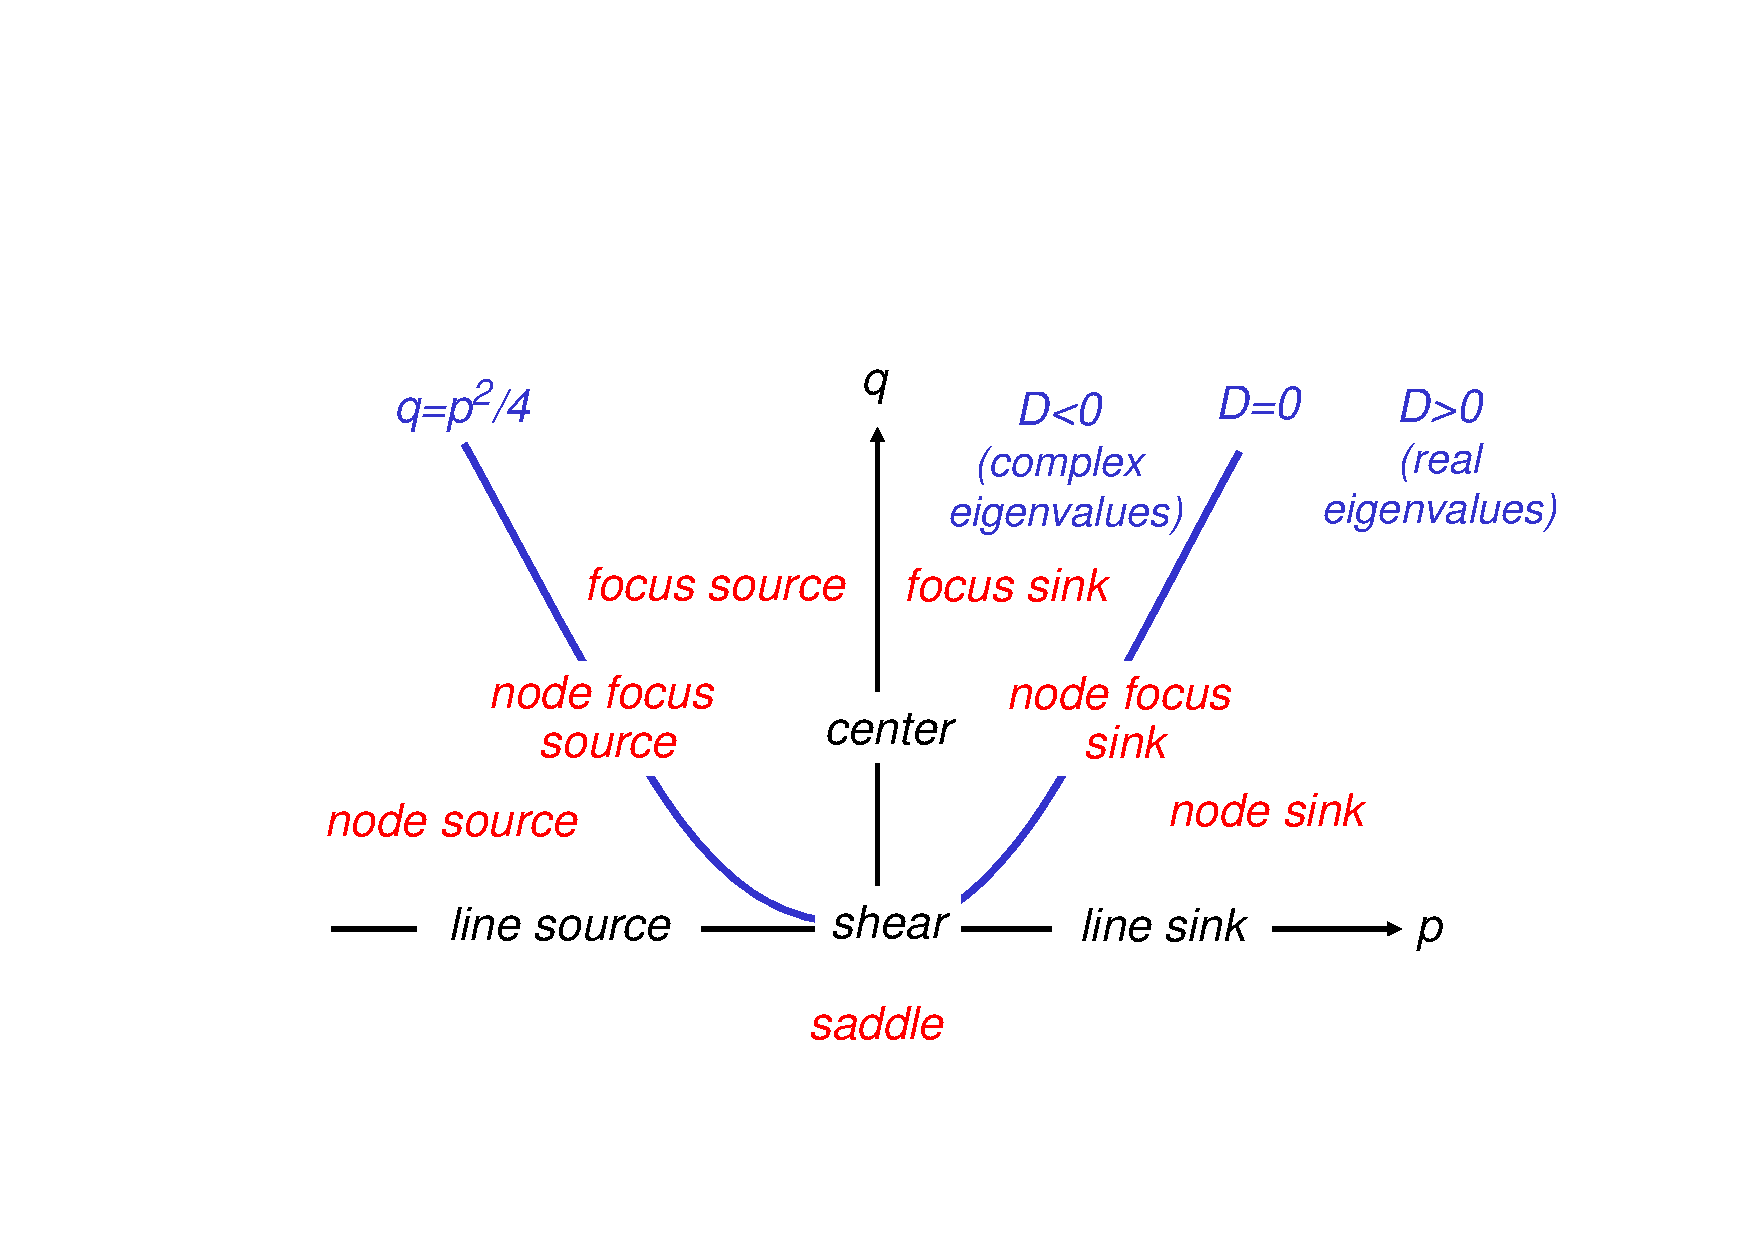
\includegraphics[width=0.8\textwidth]{img/08_pq_chart}
\end{figure}

\subsubsection{Node Source}
\begin{itemize}
    \item Positive trace
    \item Positive determinant
    \item Positive discriminant
\end{itemize}
\begin{figure}[H]
    \centering
    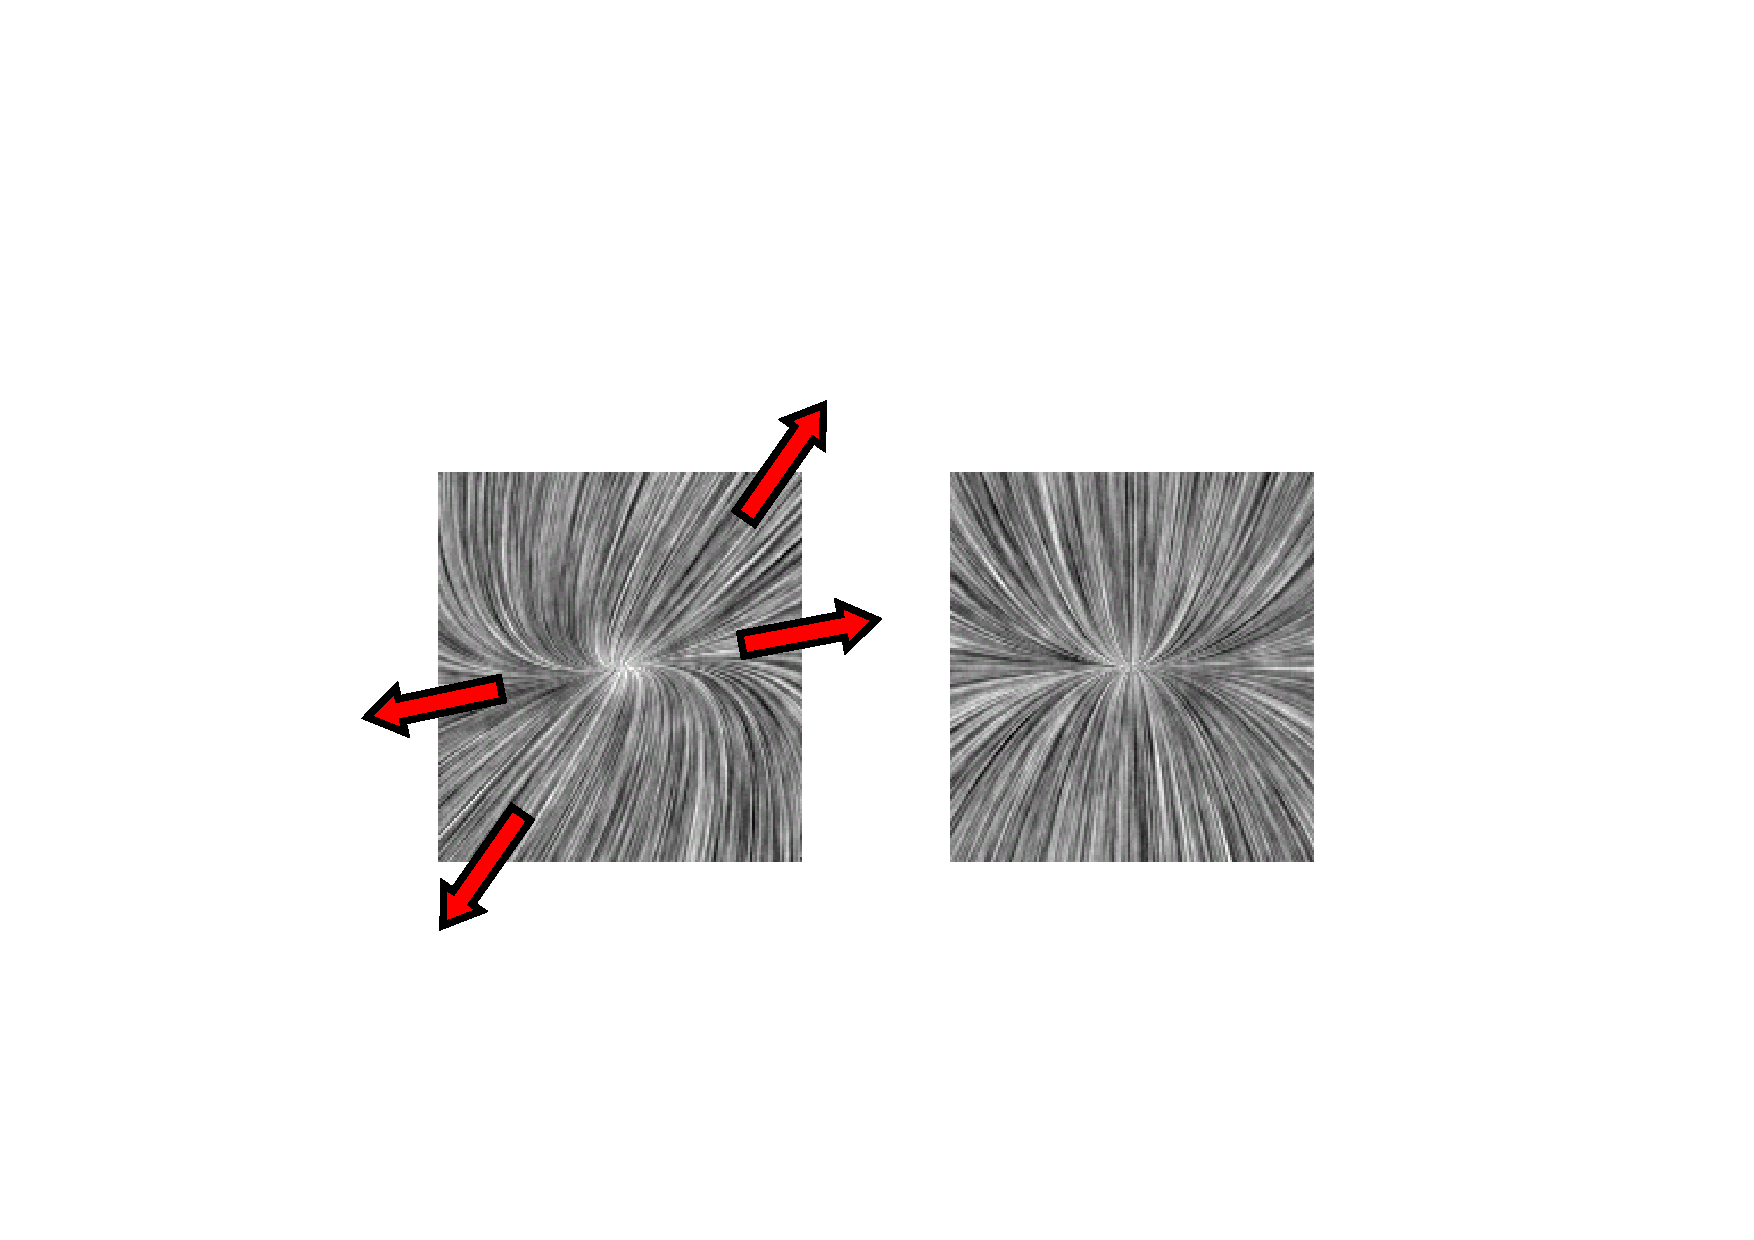
\includegraphics[width=0.6\textwidth,page=1]{img/08_2d_critical_points}
\end{figure}
\begin{align*}
J = \begin{pmatrix}
     0.425 & 0.431\\
     -0.1 & 1.075
 \end{pmatrix}
 = A ^{-1} 
     \begin{pmatrix}
         0.5 & 0\\
         0 & 1
     \end{pmatrix}A
\end{align*}

\subsubsection{Node Sink}
\begin{itemize}
    \item Negative trace
    \item Positive determinant
    \item Positive discriminant
\end{itemize}
\begin{figure}[H]
    \centering
    \includegraphics[width=0.6\textwidth,page=2]{img/08_2d_critical_points}
\end{figure}
\begin{align*}
J = \begin{pmatrix}
     -0.425 & -0.431\\
     0.1 & -1.075
 \end{pmatrix}
 = A ^{-1} 
     \begin{pmatrix}
         -0.5 & 0\\
         0 & -1
     \end{pmatrix}A
\end{align*}

\subsubsection{Saddle}
\begin{itemize}
    \item Any trace
    \item Negative determinant
    \item Positive discriminant
\end{itemize}
\begin{figure}[H]
    \centering
    \includegraphics[width=0.6\textwidth,page=3]{img/08_2d_critical_points}
\end{figure}
\begin{align*}
J = \begin{pmatrix}
     -0.434 & 1.078\\
     -0.25 & 1.15
 \end{pmatrix}
 = A ^{-1} 
     \begin{pmatrix}
         -0.25 & 0\\
         0 & 1
     \end{pmatrix}A
\end{align*}

\subsubsection{Focus Source}
\begin{itemize}
    \item Positive trace
    \item Positive determinant
    \item Negative discriminant
\end{itemize}
\begin{figure}[H]
    \centering
    \includegraphics[width=0.6\textwidth,page=4]{img/08_2d_critical_points}
\end{figure}
\begin{align*}
J = \begin{pmatrix}
     1.48 & -1.89\\
     1.04 & -0.48
 \end{pmatrix}
 = A ^{-1} 
     \begin{pmatrix}
         0.5 & -1\\
         1 & 0.5
     \end{pmatrix}A
\end{align*}

\subsubsection{Focus Sink}
\begin{itemize}
    \item Negative trace
    \item Positive determinant
    \item Negative discriminant
\end{itemize}
\begin{figure}[H]
    \centering
    \includegraphics[width=0.6\textwidth,page=5]{img/08_2d_critical_points}
\end{figure}
\begin{align*}
J = \begin{pmatrix}
     -1.48 & 1.89\\
     -1.04 & 0.48
 \end{pmatrix}
 = A ^{-1} 
     \begin{pmatrix}
         -0.5 & 1\\
         -1 & -0.5
     \end{pmatrix}A
\end{align*}


\subsubsection{Node Focus Source}
\begin{itemize}
    \item Positive trace
    \item Positive determinant
    \item Zero discriminant
\end{itemize}
Between node source and focus source (double real eigenvalue).
\begin{figure}[H]
    \centering
    \includegraphics[width=0.6\textwidth,page=6]{img/08_2d_critical_points}
\end{figure}
\begin{align*}
J = \begin{pmatrix}
     1.25 & -0.56\\
     1 & -0.25
 \end{pmatrix}
 = A ^{-1} 
     \begin{pmatrix}
         0.5 & 0\\
         1 & 0.5
     \end{pmatrix}A
\end{align*}

\subsubsection{Star Source}
Special case of the node focus source: Diagonal matrix.
\begin{figure}[H]
    \centering
    \includegraphics[width=0.6\textwidth,page=7]{img/08_2d_critical_points}
\end{figure}
\begin{align*}
J = \begin{pmatrix}
     2 & 0\\
     0 & 2
 \end{pmatrix}
 = \lambda
     \begin{pmatrix}
        1 & 0\\
         0 & 1
     \end{pmatrix}
\end{align*}

\subsection{Nonhyperbolic Critical Points}
If the eigenvalues are purely imaginary (i.e. the real parts are zero), then the critical point is the boundary case between focus source and focus sink.

This type of cricital point is called a \emph{center}. Depending on the higher derivatives it can behave as a source or as a sink. Because a center is nonhyperbolic, it is not structurally stable in general:
\begin{figure}[H]
    \centering
    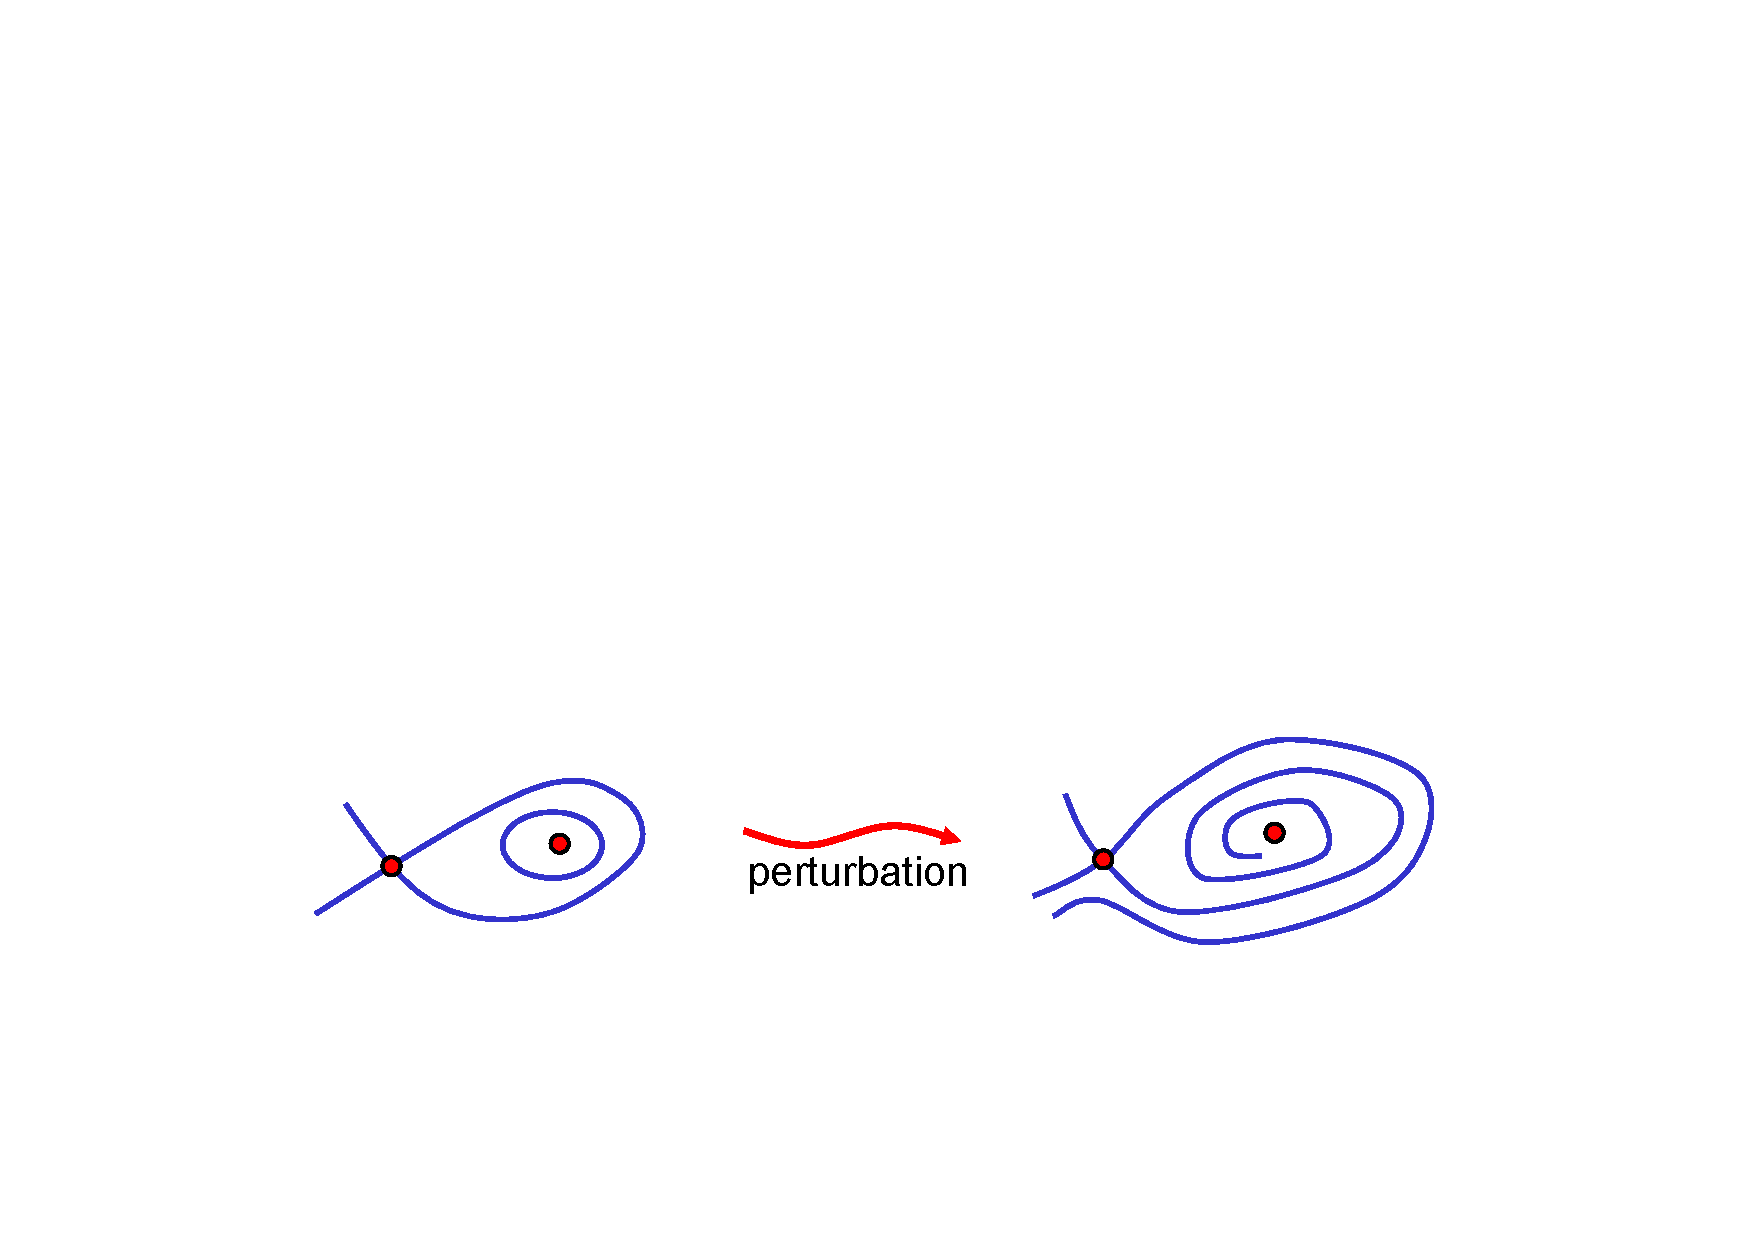
\includegraphics[width=0.6\textwidth]{img/08_nonhyperbolic_pertubation}
\end{figure}
but in the case of a \emph{divergence-free} field it is structurally stable.
\subsubsection{Center}
\begin{itemize}
    \item Zero trace
    \item Positive determinant
    \item Negative discriminant
\end{itemize}
\begin{figure}[H]
    \centering
    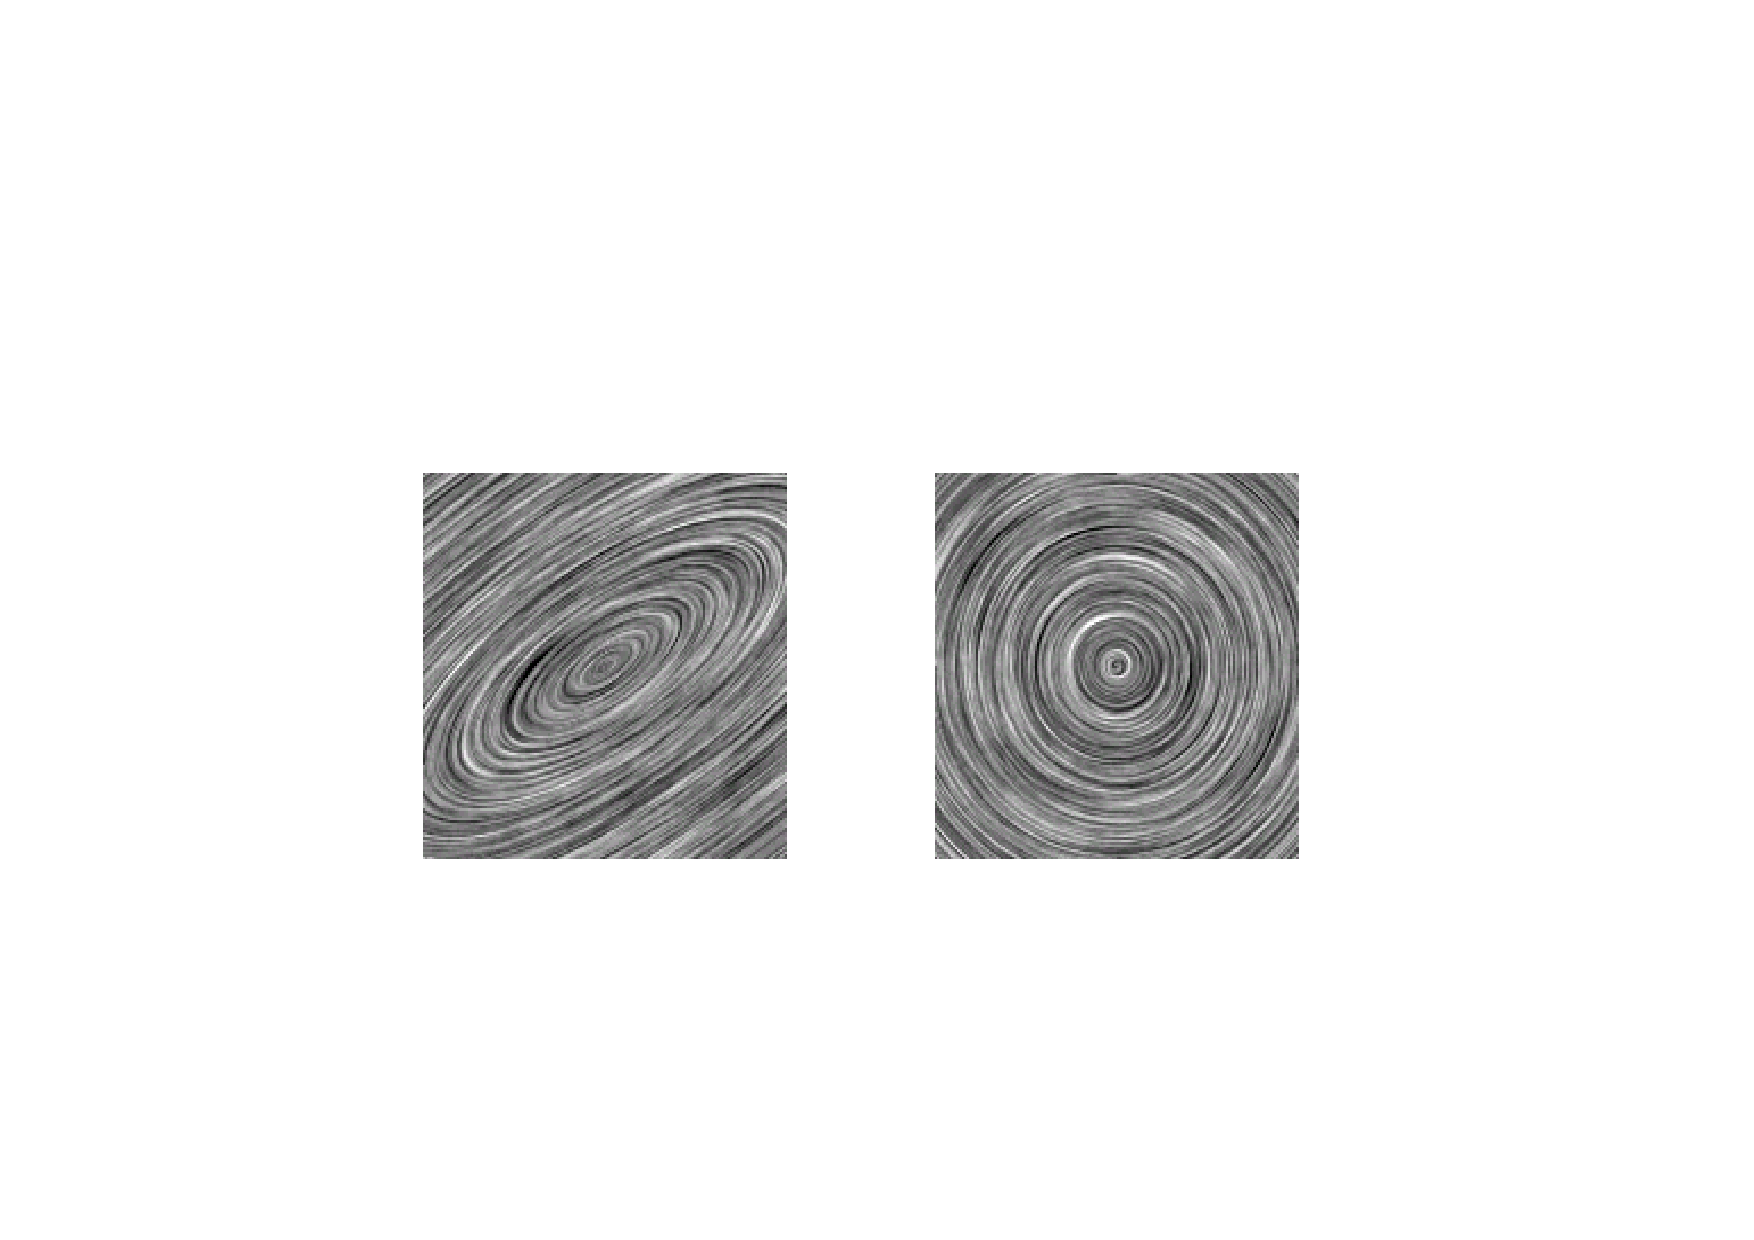
\includegraphics[width=0.6\textwidth]{img/08_center_point}
\end{figure}
\begin{align*}
J = \begin{pmatrix}
     0.98 & -1.885\\
     1.04 & -0.98
 \end{pmatrix}
 = A ^{-1} 
     \begin{pmatrix}
         0 & -1\\
         1 & 0
     \end{pmatrix}A
\end{align*}
\subsection{Other Stationary Points}
If $J$ is a singular matrix the following stationary )but not critical!) points are possible:
\begin{itemize}
    \item A single eigenvalue is zero:
    
        \emph{Line source}, \emph{Line sink}.
    \item If both eigenvalues are zero:
        
        \emph{Pure Shear}.
\end{itemize}

\subsection{The Topological Skeleton}
The \emph{topological skeleton} consists of all periodic orbits and all streamlines converging (in either direction of time) to
\begin{itemize}
    \item A saddle point (\emph{separatrix} of the saddle),
    \item A  critical point on a no-slip boundary.
\end{itemize}
It provides a kind of \emph{segmentation} of the 2D vector field.

Example:
\begin{figure}[H]
    \centering
    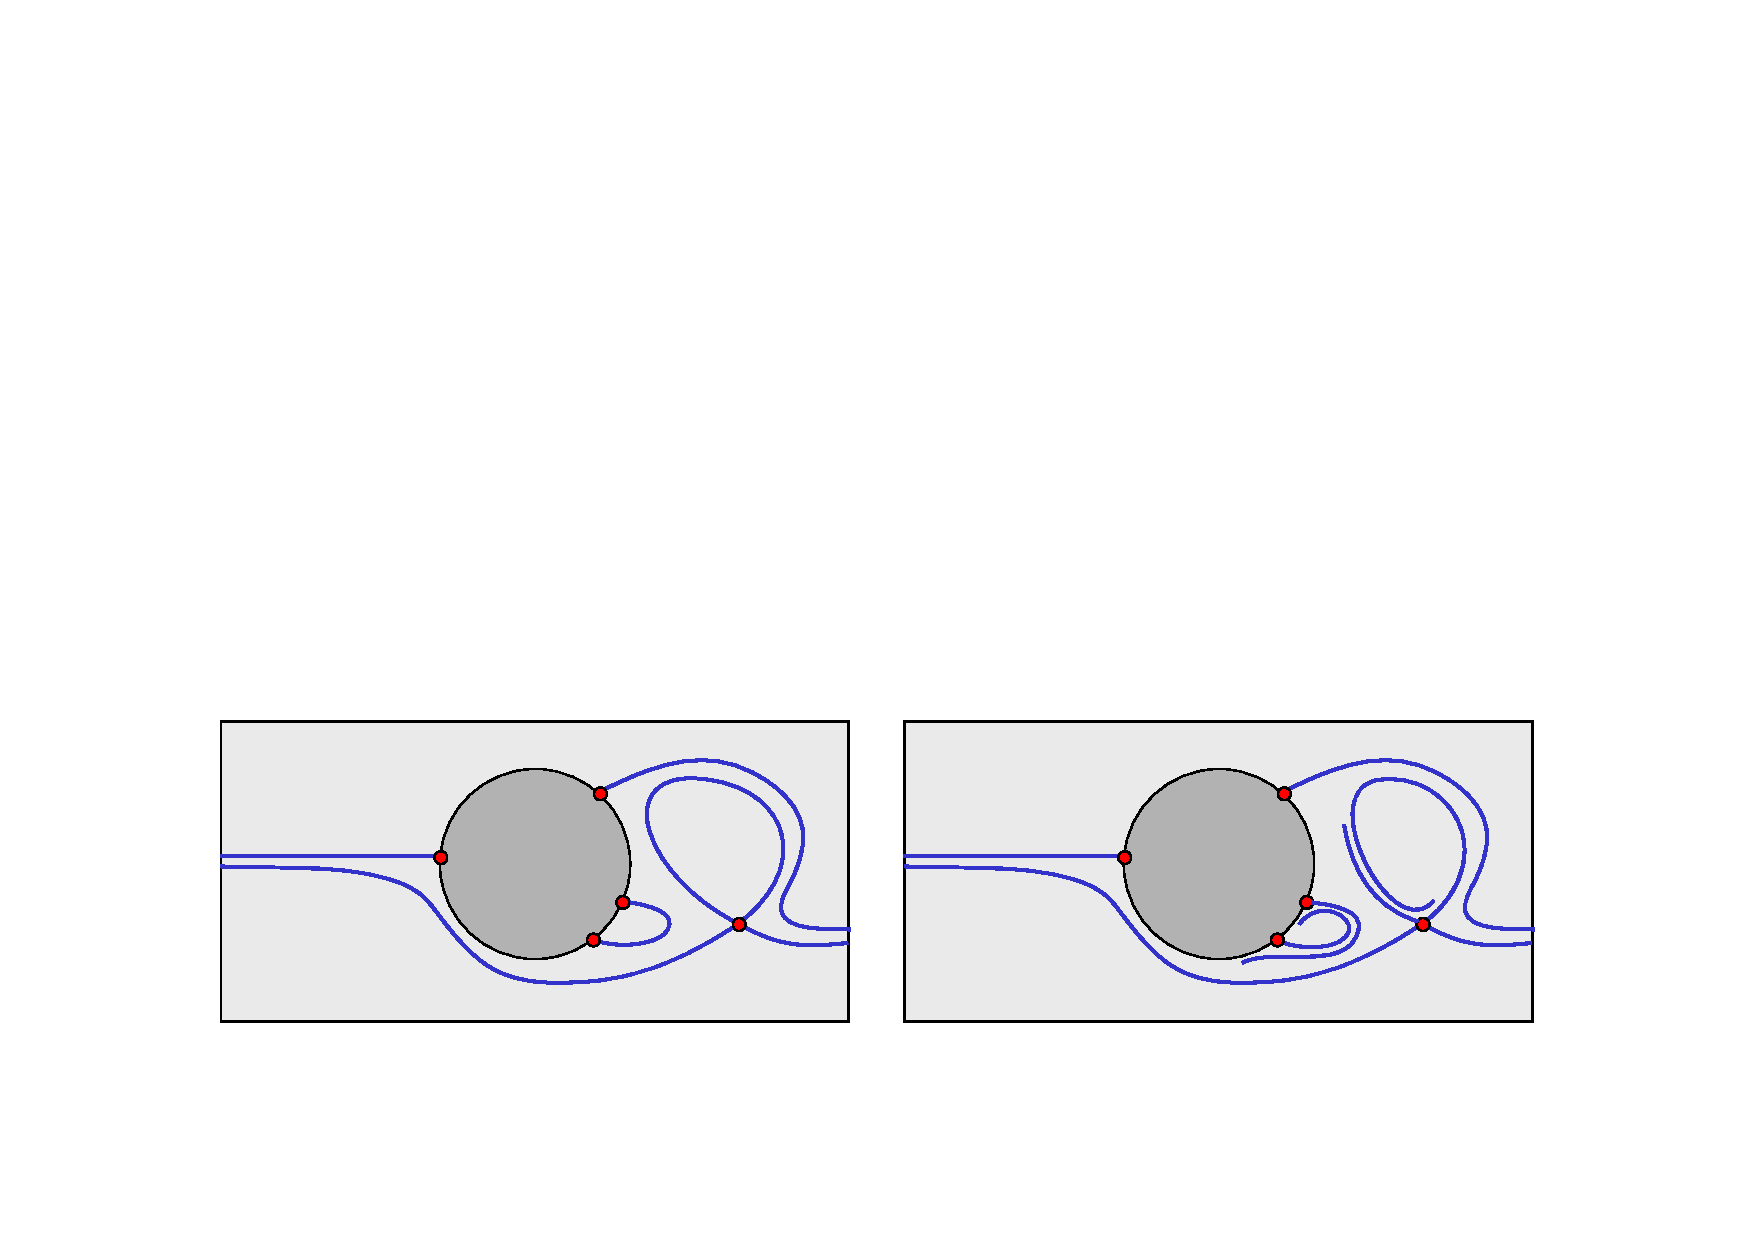
\includegraphics[width=0.7\textwidth]{img/08_topological_skeleton}
\end{figure}

\paragraph{Irrotational Vector Fields} An irrotational (conservative) vector field is the gradient of a scalar field (its potential). The skeleton of an irrotational vector field: Watershed image of its potential field. 

Discussion:
\begin{itemize}
    \item Watersheds are topologically defined and an integration is required to compute them.
    \item Height ridges are geometrically defined and locally detectable.
\end{itemize}

\subsection{Critical Points in 3D}
Hyperbolic critical points in 3D can be classified as follows:
\begin{description}
    \item Three real eigenvalues:
        \begin{itemize}
            \item All positive: \emph{Source}
            \item Two positive, one negative: 
            \emph{$1:2$ saddle} (1 in, 2 out)
            \item One positive, two negative: 
            \emph{$2:1$ saddle} (2 in, 1 out)
            \item All negative: \emph{Sink}
        \end{itemize}
    \item One real, two complex eigenvalues:
        \begin{itemize}
            \item Positive real eigenvalue, positive real parts: \emph{Spiral source}
            \item Positive real eigenvalue, negative real parts: \emph{$2:1$ Spiral saddle}
            \item Negative real eigenvalue, positive real parts: \emph{$2:1$ Spiral saddle}
            \item Negative real eigenvalue, negative real parts: \emph{Spiral sink}
        \end{itemize}

\end{description}

\begin{figure}
    \centering
    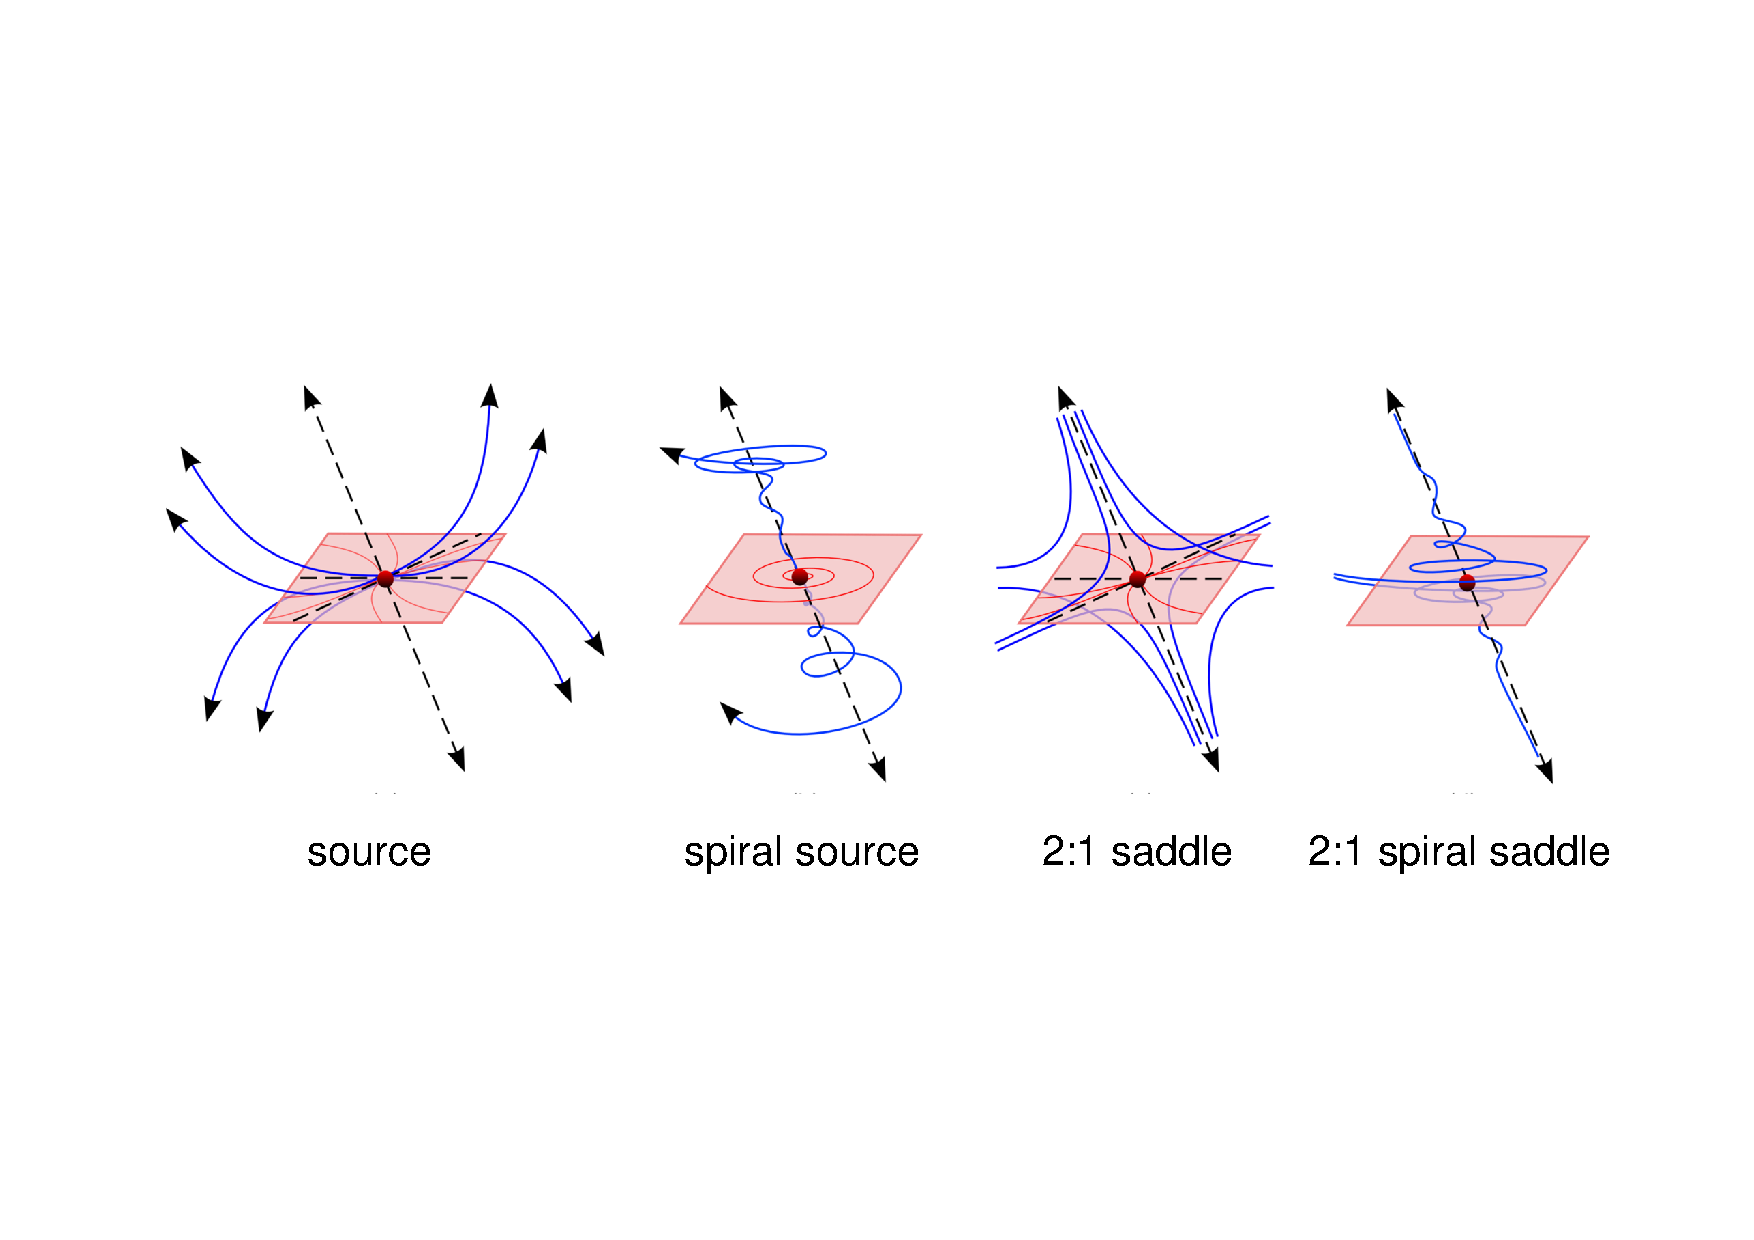
\includegraphics[width=0.8\textwidth]{img/08_3d_critical_points}
\end{figure}


\subsection{Periodic Orbits}
The \emph{Poincaré map} of a periodic orbit in 3D:
\begin{itemize}
    \item Choose a point $x_0$ on the periodic orbit.
    \item Choose an open circular disk $D$ centered at $x_0$ on a plane which is not tangential that is \emph{not tangential} to the flow and small enough that the periodic orbit intersects $D$ only in $x_0$.
    \item Any streamline seeded at a point $x\in D$ intersects $D$ the next time at a point $x' \in D$ defines a mapping from $x$ to $x'$.
    \item There exists a smaller open disk $D_0\subseteq D$ centered at $x_0$ such that this mapping is defined for all points $x\in D_0$.
    \item This is the Poincaré map.
        \begin{figure}[H]
            \centering
            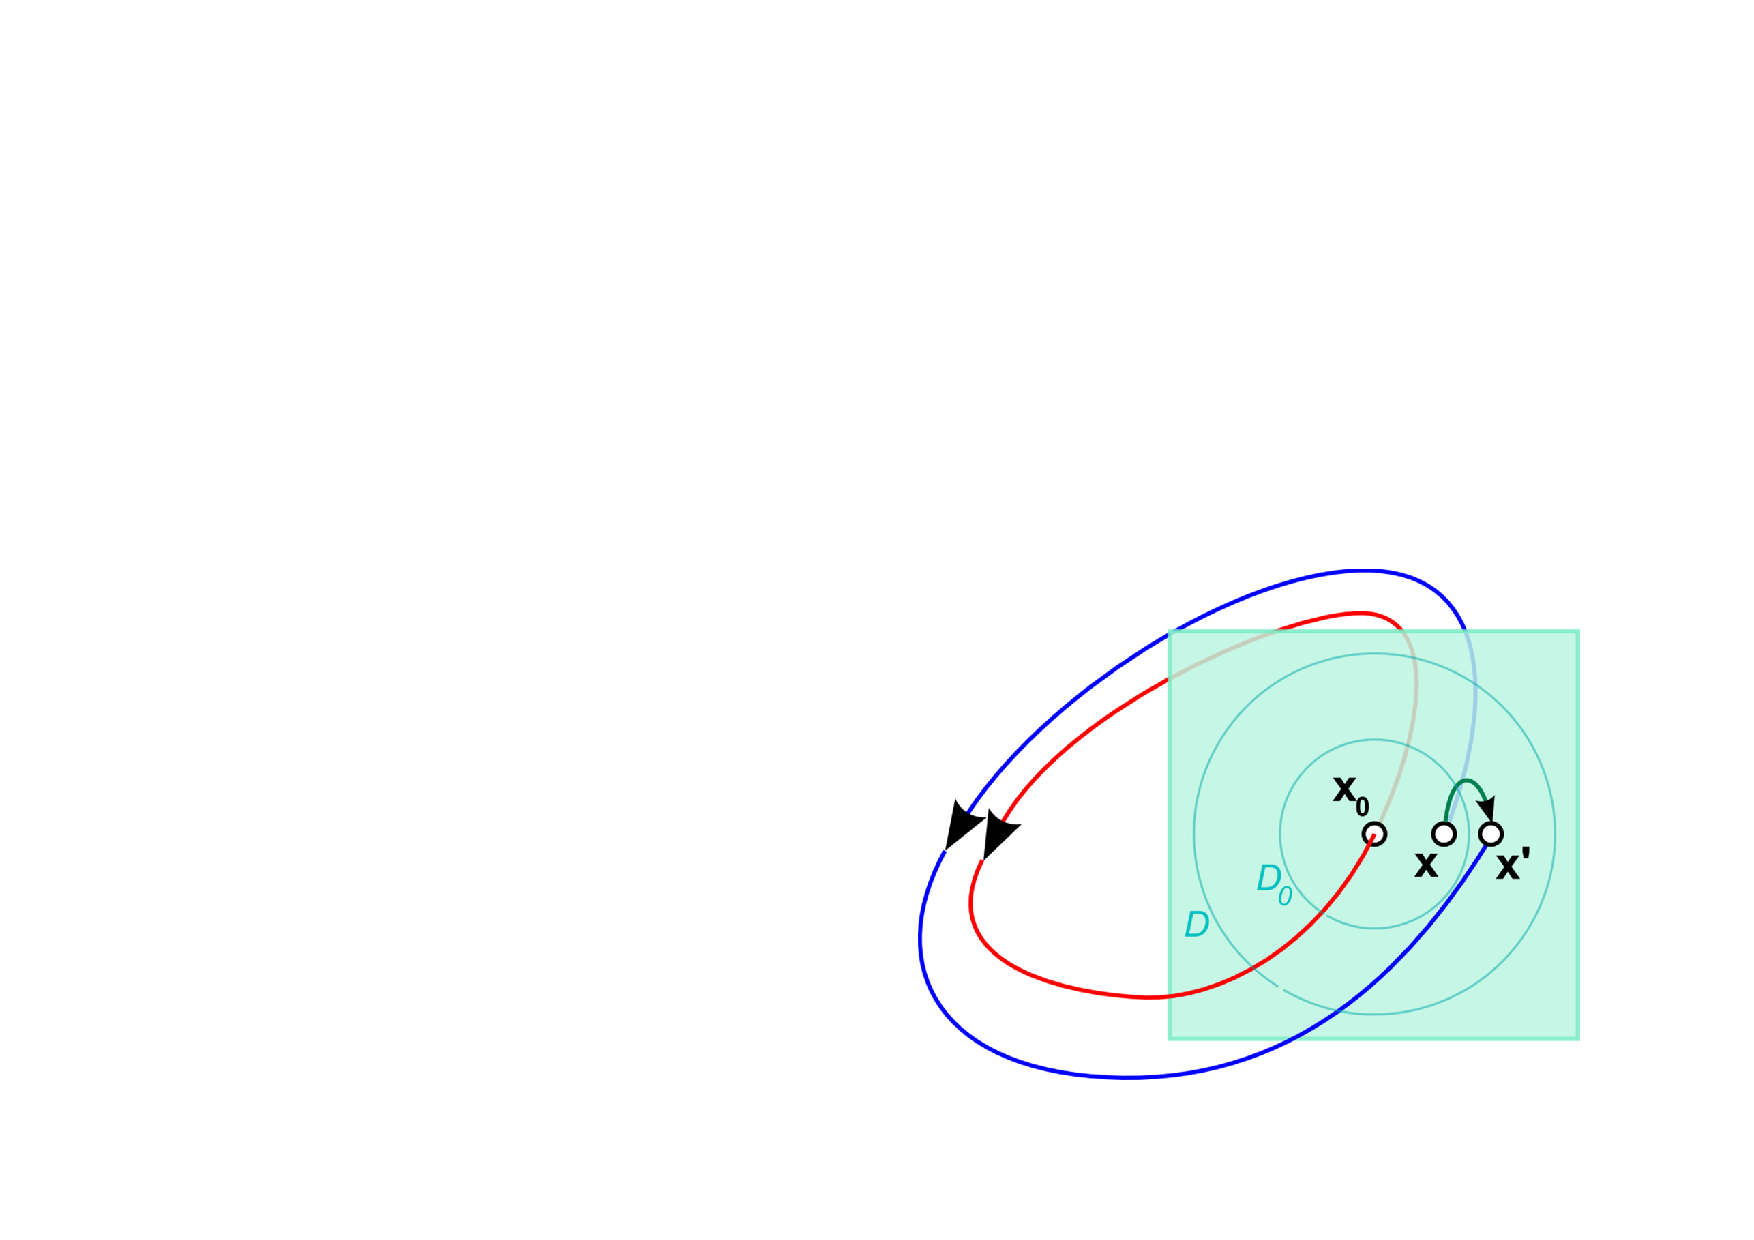
\includegraphics[width=0.6\textwidth]{img/08_poincare_map}
        \end{figure}
        
\end{itemize}

Using the coordinates on the plane of $D$ and with origin at $x_0$ the Poincaré map can now be linearised:
    \begin{align*}
        x\mapsto Px
    \end{align*}
where $P$ is a $2\times 2$ matrix.

Important facts about Poincaré maps: The eigenvalues of $P$ are independent of
\begin{itemize}
    \item The choice of $x_0$ on the periodic orbit,
    \item The orientation of the plane of $D$,
    \item The choice of coordinates for the plane.
\end{itemize}

A periodic orbit is called \emph{hyperbolic} if its eigenvalues \emph{lie off the complex unit circle}. Hyperbolic periodic orbits are structurally stable.

Types of hyperbolic orbits in 3D:
\begin{figure}[H]
    \centering
    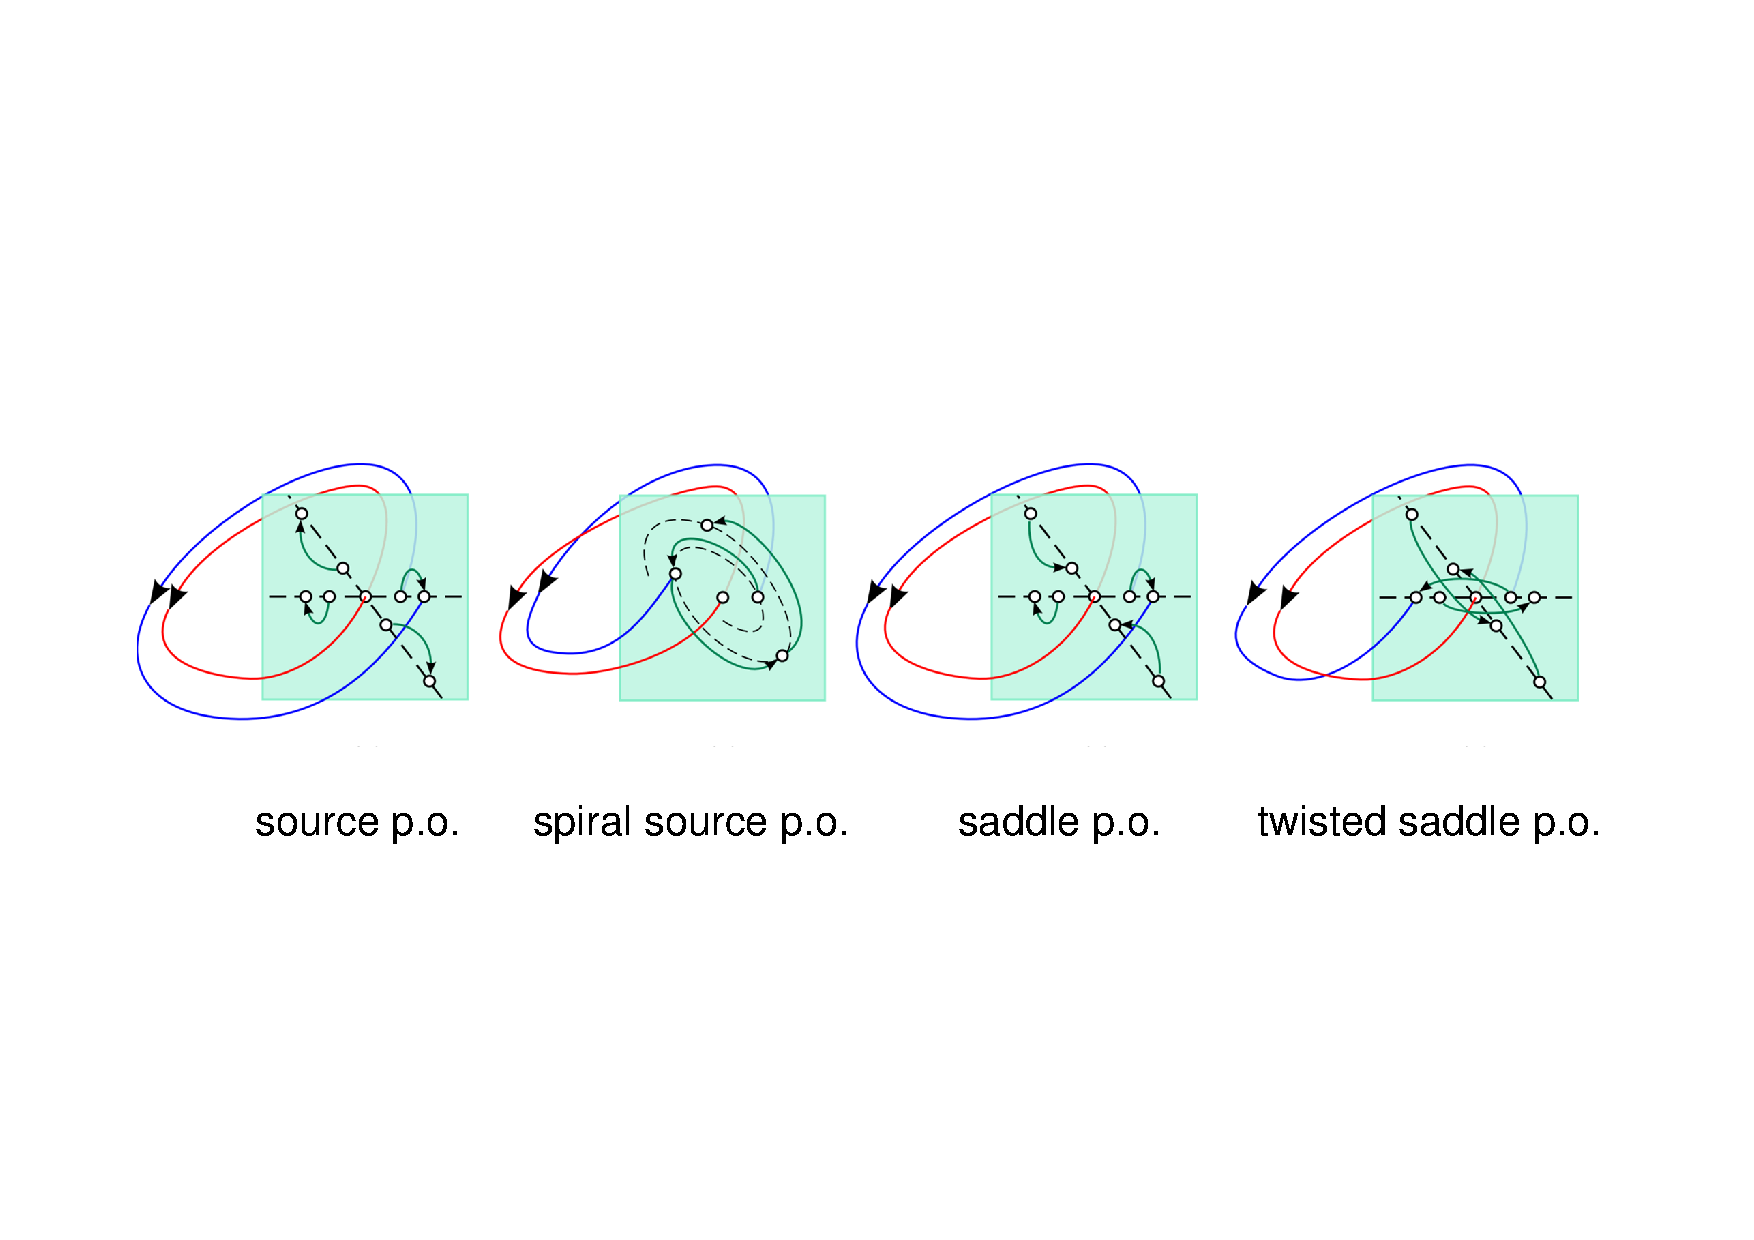
\includegraphics[width=0.8\textwidth]{img/08_periodic_orbits}
\end{figure}

\subsection{Saddle Connectors}
The topological skeleton of 3D vector fields contains 1D and 2D separatrices of (spiral) saddles. 

This is not directly usable for visualisation (too much ooclusion). Alternative: Only show \emph{intersection curves} of 2D separatrices.

Two types of saddle connectors:
\begin{description}
    \item \emph{Heteroclinic orbits}: Connects two (spiral) saddles
    \item \emph{Homoclinic orbits}: Connects a (spiral) saddle with itesld.
\end{description}


In rotational flow, a connected pair of spiral saddles can describe a \emph{vortex breakdown bubble}.
\begin{description}
    \item Ideal case:    
        \begin{itemize}
            \item $W_S(P_1)$ coincides with $W_u(P_2)$
            \item No saddle connector
        \end{itemize}
    \item Perturbed case:
        \begin{itemize}
            \item Transversal intersection of $W_S(P_1)$ and $W_U(P_2)$
            \item Saddle connector consists of two streamlines
        \end{itemize}
\end{description}
\begin{figure}[H]
\centering
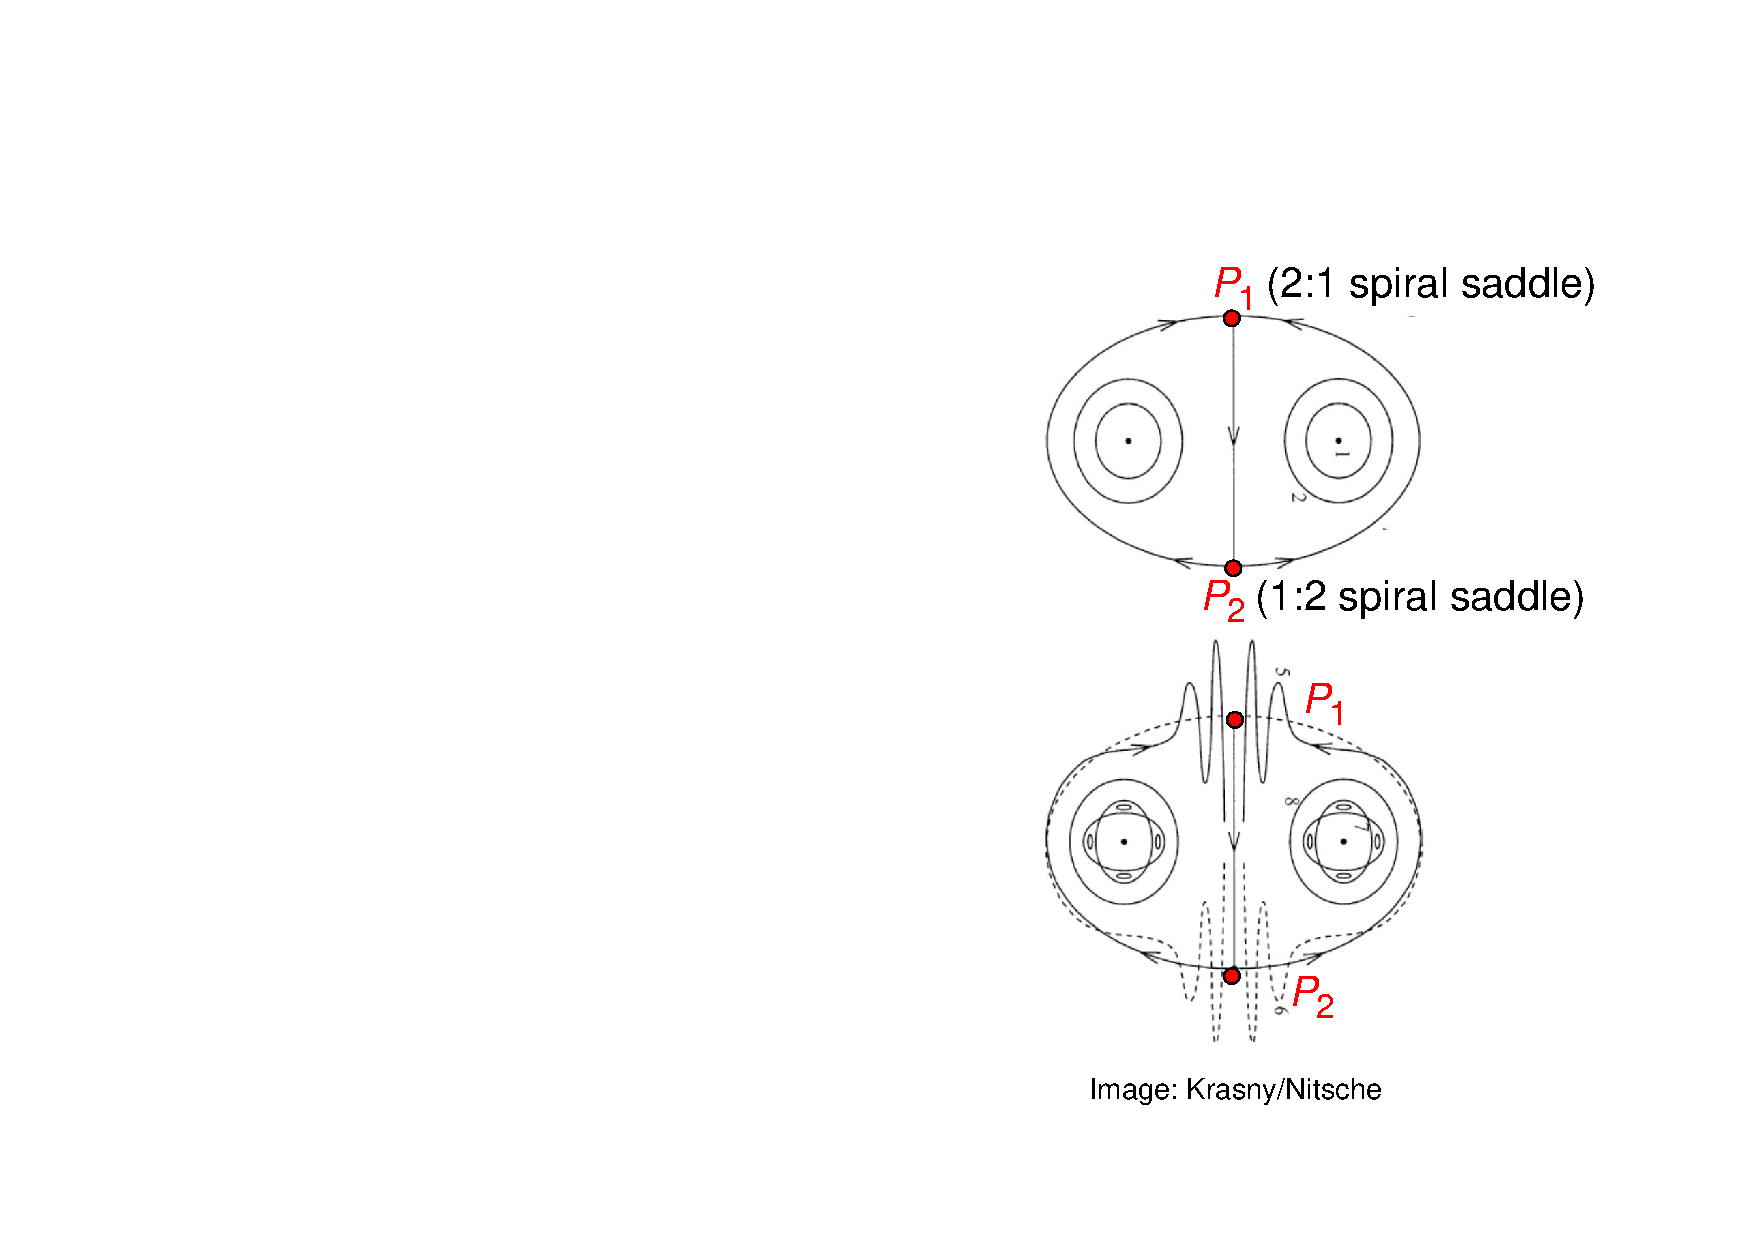
\includegraphics[width=0.4\textwidth]{img/08_saddle_connectors}
    \caption{Top: Ideal case, Bottom: Perturbed case}
\end{figure}

Pair of spiral saddles, 3D view:
\begin{figure}[H]
\centering
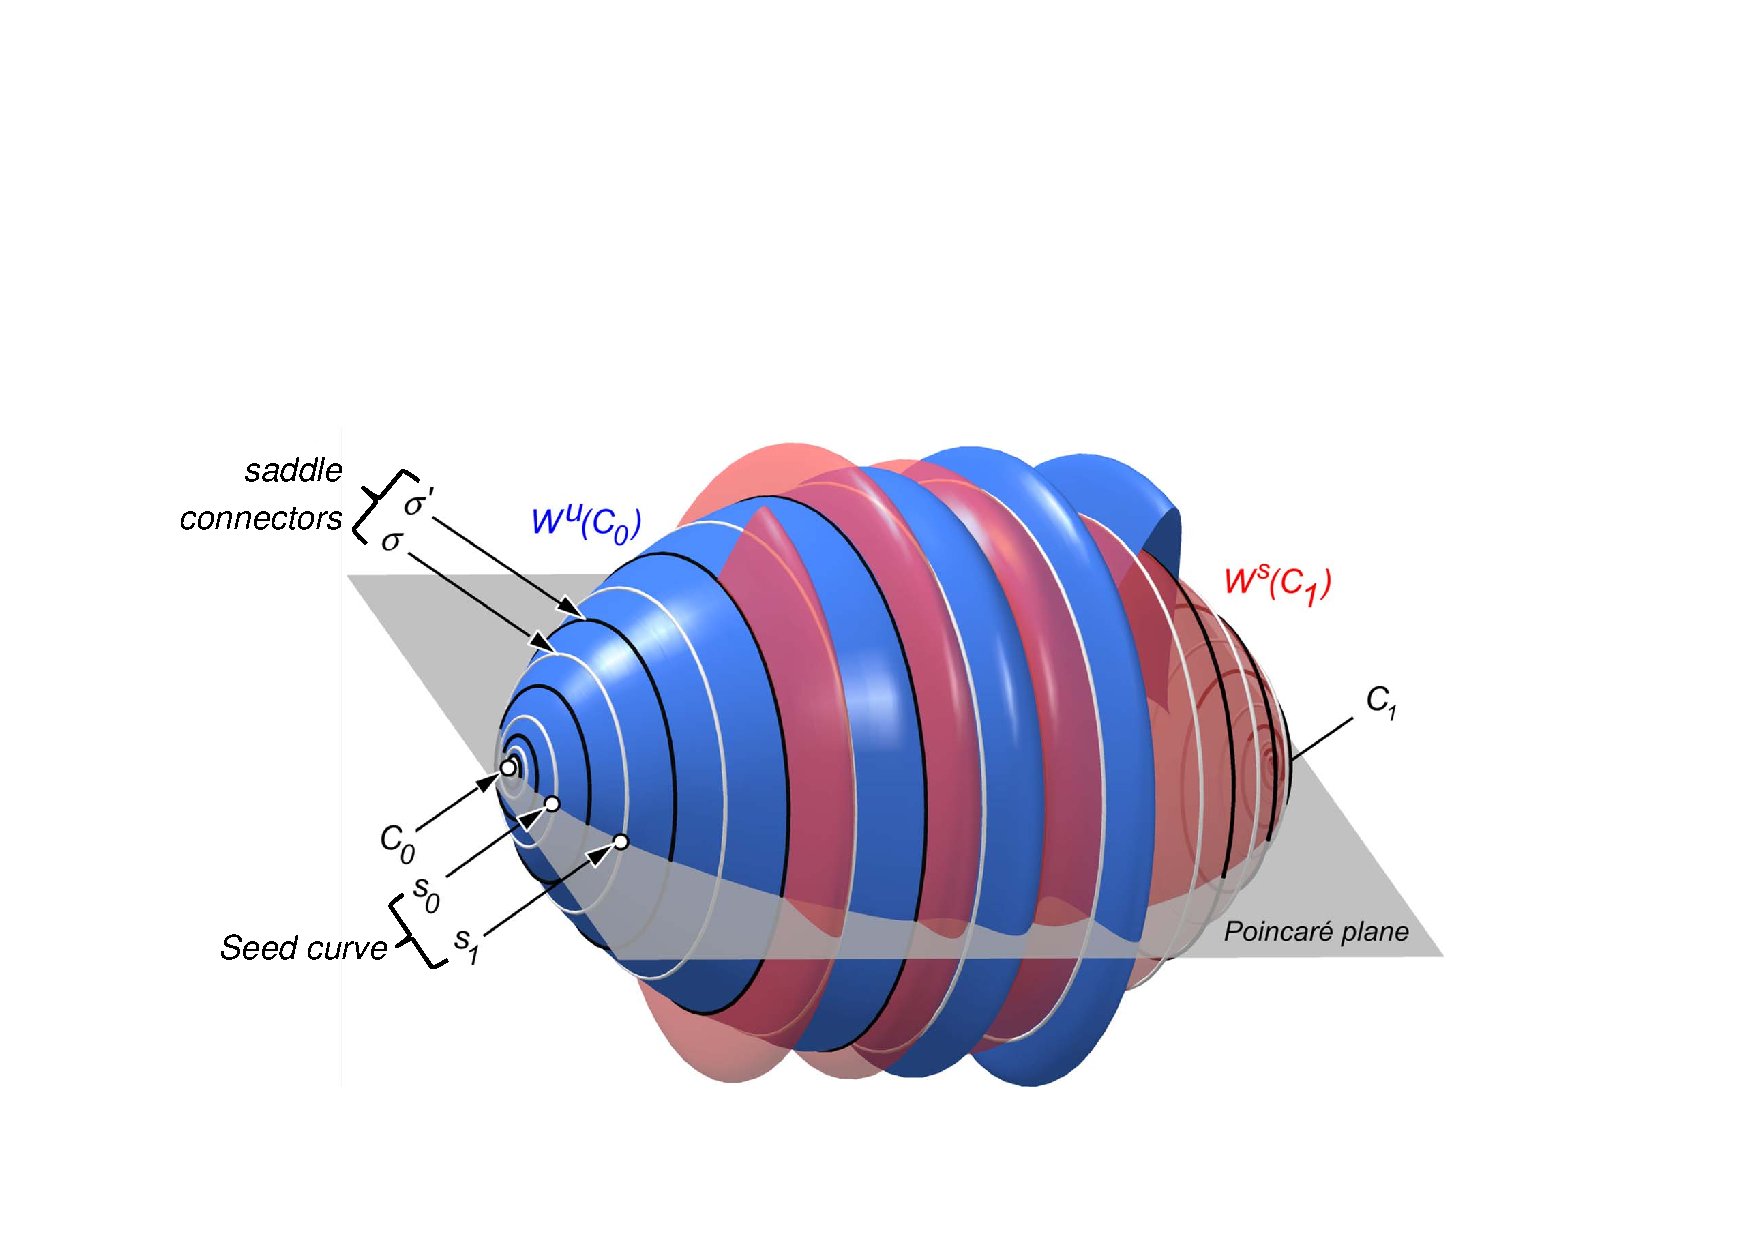
\includegraphics[width=0.8\textwidth]{img/08_pair_spiral_saddles}
\caption{Perturbed saddle connector connecting $C_0$ and $C_1$}
\end{figure}

If $v$ is the velocity field of a fluid: Folds must have a constant mass flux. Close to $P_1$ or $P_2$ this is approximately
\begin{align*}
    \int \rho v\ dn &\approx \rho \omega A r &(\text{density $\cdot$ angular velocity $\cdot$ cross section area $\cdot$ radius})
\end{align*}


























